% Chapter Template

\chapter{Deep Learning} % Main chapter title

\label{Chapter4} % Change X to a consecutive number; for referencing this chapter elsewhere, use \ref{ChapterX}

Deep learning experiences a renaissance because of the technology improvements in hardware and software. The collection of data has also significant improved making it possible to train even more complex models. The purpose of supervised Deep Learning is to learn a relationship between input and output:
$$Y=f(X) + \epsilon$$



%----------------------------------------------------------------------------------------
%	SECTION 1
%----------------------------------------------------------------------------------------

\section{Deep learning teory}
Deep Learning is a specialized field in Machine Learning, which means it is within the field of applied statistics. Like in statistics and Machine Learning the basic components of a Deep Learning algorithm are a dataset, cost function, optimazation algorithm and a model. E.g. in the lsm method we assumed the model was Gaussian, dataset was the simulated paths, the lose function was the mean square error and the optimazation algorithm was solving the normal equations. Deep learning is about studying neural networks which allows for greater flexiblity than standard methods like linear regression. "Deep" comes from that a neural network consists of multiple layers, where the depth tells you how many layers the network has. The network consists of a input layer, hidden layers and finally a output layer where the input and output layers are observable to the user. To fit a model we need to provide weights, bias and the activation function for each layer, hence the ouput is a chain of functions applied to the input. In order to measure the performance of the model, we need a function to measure the difference on the response variable and the actually observed response. This function is referred as the loss function, where the cost function is the average over the loss functions. The cost function tells us how good our model is on the data. The cost function is key to improving our model or in machine learning lingo learning the model, hence we applied an optimization algorithm to find the optimal set of weights in order to improve the cost function \parencite{Goodfellow-et-al-2016}.

%-----------------------------------
%	SUBSECTION 1
%-----------------------------------
\subsection{Architecture}
The neural network is not like classical linear regression in section \ref{LSM} where a single linear transformation from input to output is applied. In neural network we have a larged nested function, where each input go through a chain of functions until reaching the output. Each function in the composition of functions correspond to a "layer" in the neural network. The neural network inputs are called the input layer, the output layer is the output of the neural network. The layers between the input and output layer are hidden layers. This could be an explanation why the field is called Deep learning, because we a deep structure of layers. Each layer consists of neurons, where the width of the layer is the number of neurons (see figure \ref{fig:DNN}).

\usetikzlibrary{matrix,chains,positioning,decorations.pathreplacing,arrows}
\usetikzlibrary{positioning,calc}
\tikzset{%
  every neuron/.style={circle,draw,minimum size=1cm},
  neuron missing/.style={draw=none,scale=4,text height=0.333cm,execute at begin node=\color{black}$\vdots$},
}
\begin{center}
    \begin{figure}[th]
        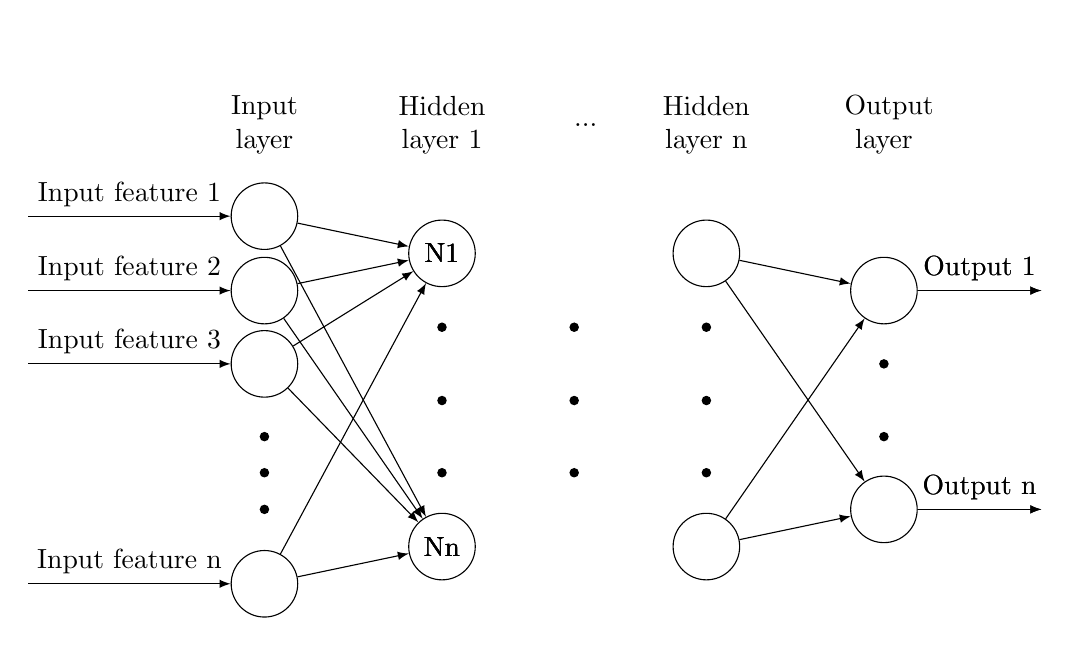
\begin{tikzpicture}[
            plain/.style={
              draw=none,
              fill=none,
              },
            dot/.style={draw,shape=circle,minimum size=3pt,inner sep=0,fill=black
              },
            net/.style={
              matrix of nodes,
              nodes={
                draw,
                circle,
                inner sep=8.5pt
                },
              nodes in empty cells,
              column sep=0.1cm,
              row sep=-11pt
              },
            >=latex
            ]
            \matrix[net] (mat)
            {
            |[plain]| \parbox{1cm}{\centering Input\\layer} 
                        & |[plain]| \parbox{1.2cm}{\centering Hidden\\layer 1} 
                                    &  |[plain]| \parbox{0cm}{\centering ...} 
                                                &  |[plain]| \parbox{1.2cm}{\centering Hidden\\layer n} 
                                                                & |[plain]| \parbox{1cm}{\centering Output\\layer} \\
                        & |[plain]| & |[plain]| & |[plain]|     & |[plain]|                                   \\
            |[plain]|   &           & |[plain]| &               & |[plain]|    \\
                        & |[plain]| & |[plain]| & |[plain]|     &              \\
            |[plain]|   & |[dot]|   & |[dot]|   & |[dot]|                 \\
                        & |[plain]| & |[plain]| & |[plain]|     & |[dot]|      \\
            |[plain]|   & |[dot]|   & |[dot]|   & |[dot]|       & |[plain]|    \\
            |[dot]|     & |[plain]| & |[plain]| & |[plain]|     & |[dot]|      \\
            |[dot]|     & |[dot]|   & |[dot]|   & |[dot]|       & |[plain]|    \\
            |[dot]|     & |[plain]| & |[plain]| & |[plain]|     &              \\
            |[plain]|   &           & |[plain]| &               & |[plain]|    \\
                        & |[plain]| & |[plain]|            \\
            };
            \foreach \ai/\mi in {2/Input feature 1,4/Input feature 2,6/Input feature 3,12/Input feature n}
              \draw[<-] (mat-\ai-1) -- node[above] {\mi} +(-3cm,0);

            \foreach \ai in {2,4,6,12}
            {\foreach \aii/\mii in {3/N1,11/Nn}
                \draw[->] (mat-\ai-1) -- (mat-\aii-2) node[yshift=0cm] {\mii};
            }
            \foreach \ai in {3,11}
            {  
                \draw[->] (mat-\ai-4) -- (mat-4-5);
                \draw[->] (mat-4-5) -- node[above] {Output 1} +(2cm,0);\
            }
            \foreach \ai in {3,11}
            {
                \draw[->] (mat-\ai-4) -- (mat-10-5);
                \draw[->] (mat-10-5) -- node[above] {Output n} +(2cm,0);
            }
        \end{tikzpicture}
        \caption{Deep Neural Network structure.}
        \label{fig:DNN}
    \end{figure}
\end{center}

Dense layers

%-----------------------------------
%	SUBSECTION 2
%-----------------------------------
\subsection{Forward propagation}
activation function important feature for neural network, why are they used?
activation functions apply a non-linear transformation and decide whether a neuron should be activated or not. Without activation functions the whole network would essentially be a linear regression model.
variations:
\begin{enumerate}
\item[•] Sigmoid function: $f(x)=\frac{1}{1+\exp(-x)}$
\item[•] Hyperbolic tangent function: scaled and shifted sigmoid function: $f(x)=\frac{2}{1+\exp(-2x)} - 1$ (good for hidden layers)
\item[•] ReLU function most popular choice $f(x)=\max(0,x)$. Rule of thump use ReLU
\item[•] Leaky ReLU function better version than Relu:  \[ f(x)=
    \begin{dcases}
        x & if \ x \geq 0 \\
        a\cdot x & otherwise \\
    \end{dcases}
\] (try to solve the vanishing gradient problem (weights will not be update/neuron are dead))
\item[•] Softmax function: $S(y_i)=\frac{\exp(y_i)}{\sum_{i=1}^{n}\exp(y_i)}$
\end{enumerate}

These network of models are called feedforward because the information only travels forward in the neural network, through the input nodes then through the hidden layers (single or many layers) and finally through the output nodes. 
%-----------------------------------
%	SUBSECTION 3
%-----------------------------------

\subsection{Optimization}
Quantifying loss
Gradients is essential for model optimization
stepwidth is our learning rate

\subsection{Backpropagation}
The chain rule: $\frac{dz}{dx}= \frac{dz}{dy} \frac{dy}{dx}$
coputational graph - local gradient -> gradient, because we want to minimize the loss function
so we want $\frac{\partial Loss}{\partial x}$ use chain rule to find the "final gradient".
SO three steps:
1. forward pass: compute Loss
2. compute local gradients
3. backward pass: compute $\dfrac{\partial Loss}{\partial weights}$ using chain rule


%----------------------------------------------------------------------------------------
%	SECTION 2
%----------------------------------------------------------------------------------------

\section{Deep Learning And Option Pricing}

The unique attribute of neural network is the ability to approximate any kind of function (Universal Apporximate Theorem), because of the flexiblility with applying multiple functions to the input layer. The neural network has a lot of different design options, where e.g. hidden layers, layer width, activation functions etc. are hyperparameters.